% ===================== PARTE 9: TOPOLOGÍA Y AFINIDAD (nueva) =====================
\parte{Topología y afinidad}{Topología y afinidad:\\¿importa dónde cae cada hilo?}
  {Los mismos 4 hilos, cada vez más lejos; dos hilos en cada pareja de núcleos; y la miniatura frente al original.}{p9_portada}

\begin{frame}{Los mismos 4 hilos, cada vez más lejos}
  \fuente{docker/rendimiento.csv, colocaciones E4-compacto, E4-disperso y P4; EXPLICACION.md, Parte 6.4}
  \begin{columns}[T]
    \column{0.66\textwidth}
    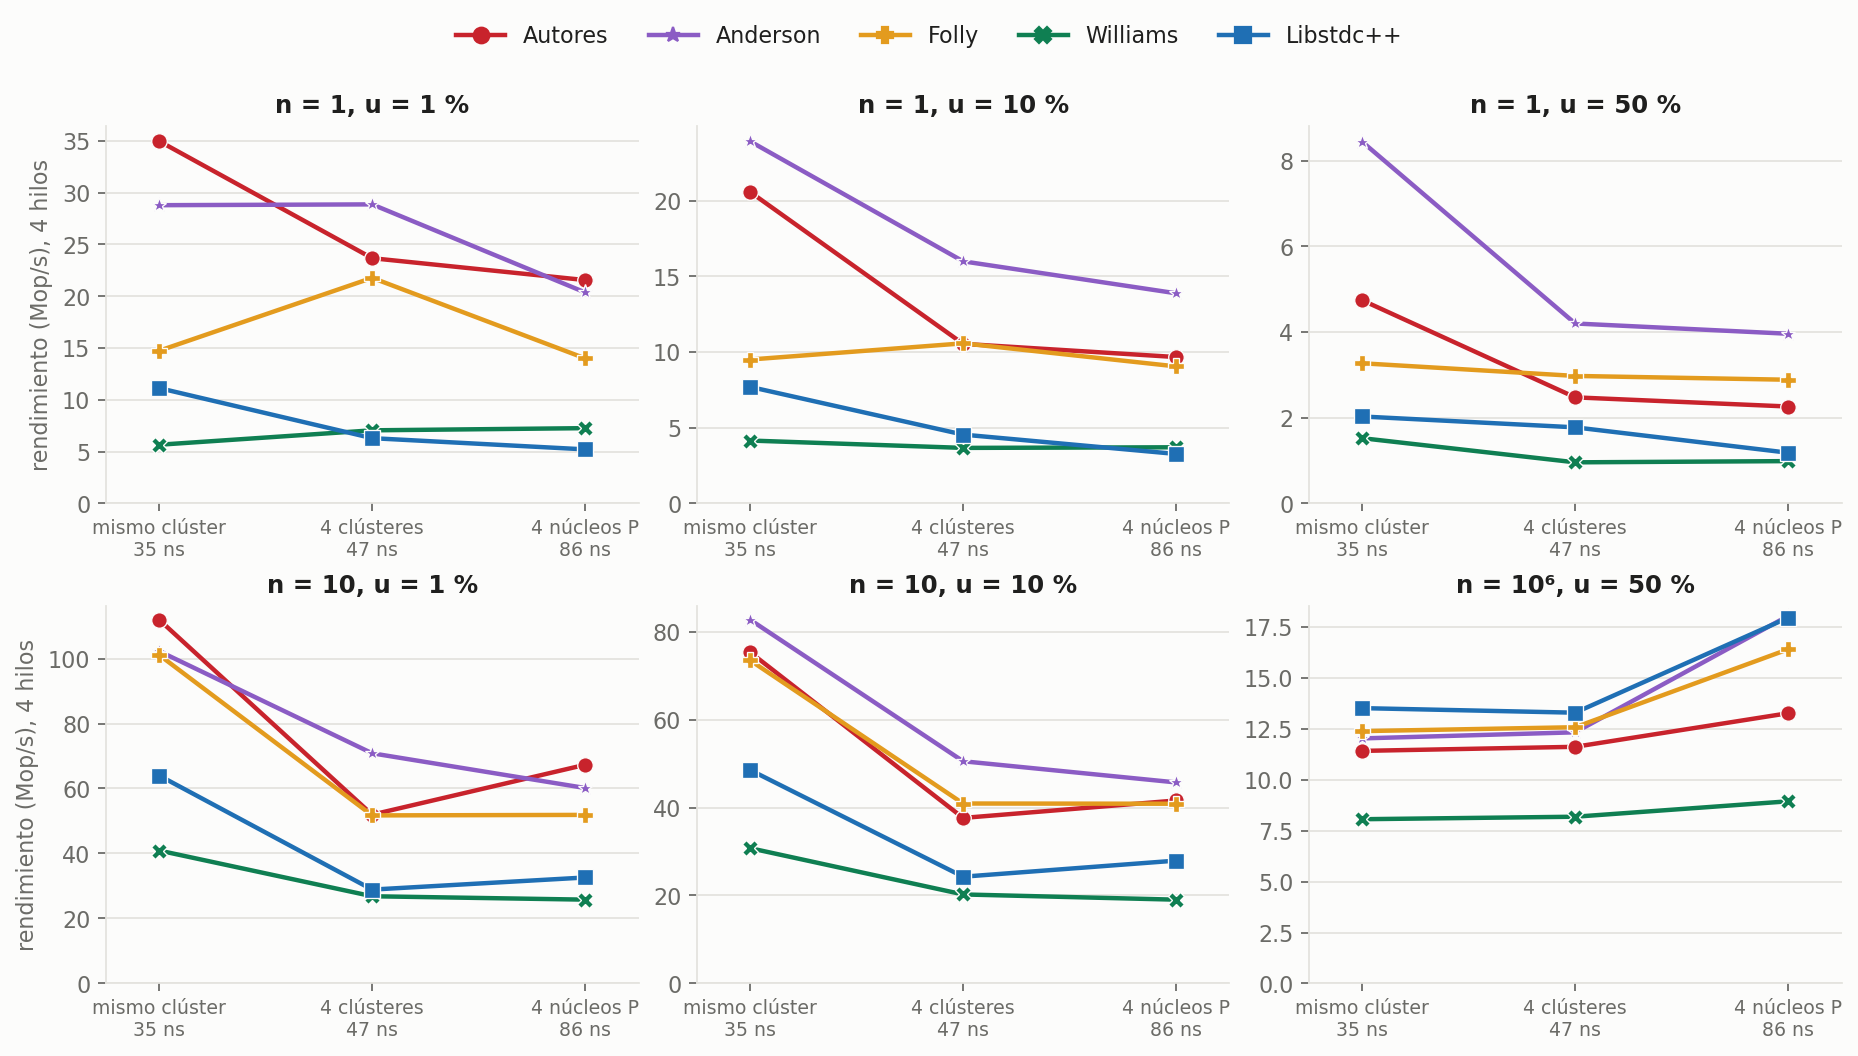
\includegraphics[width=\linewidth]{figuras/afinidad_dosis_respuesta}
    \column{0.3\textwidth}
    \caja{En cada panel, de izquierda a derecha: los 4 hilos en un clúster (35\,ns por viaje), uno en cada clúster (47\,ns) y 4 núcleos P (86\,ns).}
    \par\medskip
    \caja{Con contención, las líneas bajan al separar los hilos. Con $n = \pot{6}$ casi no se mueven: es el control.}
  \end{columns}
  \nota{p9_dosis}
\end{frame}

\begin{frame}{Separar cuesta mucho donde hay contención, y nada donde no}
  \fuente{docker/rendimiento.csv; tablas.md, «Efecto de separar los hilos entre sockets»; EXPLICACION.md, Parte 6.4}
  \begin{columns}[T]
    \column{0.56\textwidth}
    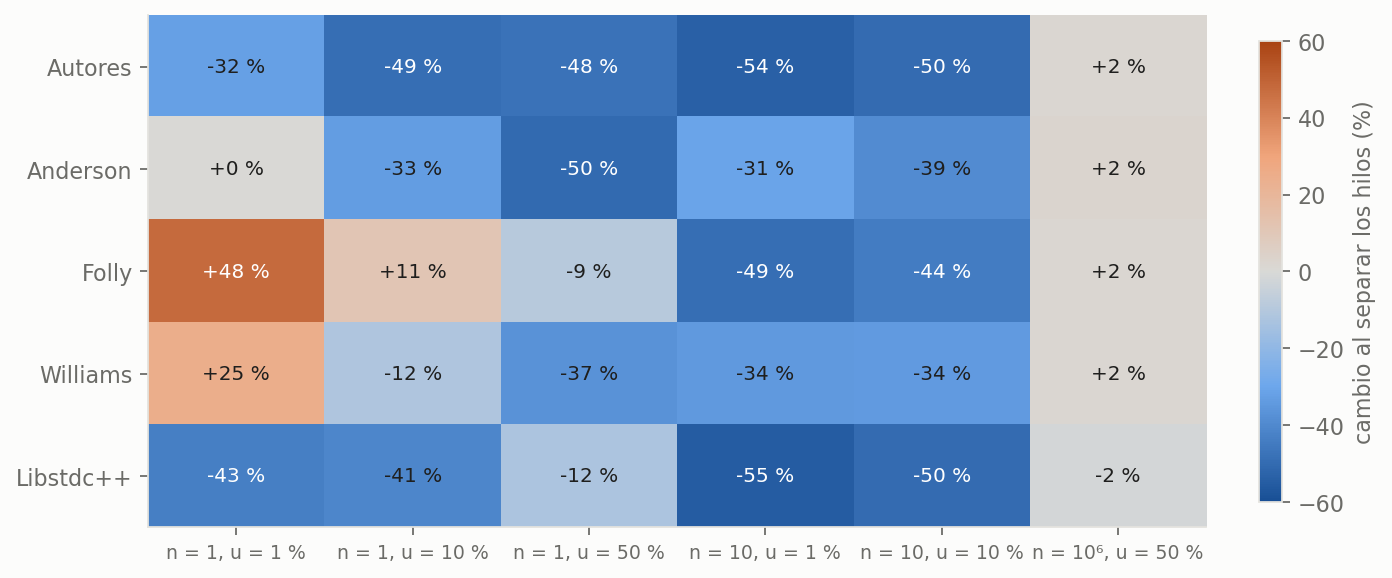
\includegraphics[width=\linewidth]{figuras/afinidad_mapa_4hilos}
    \par\scriptsize\color{gris} Cambio al pasar de 1 clúster a 4 clústeres, solo núcleos E. Azul: pierde al separar; naranja: gana.
    \column{0.4\textwidth}
    \begin{enumerate}\footnotesize\setlength{\itemsep}{3pt}
      \item \textbf{Con contención, cuesta mucho:} Autores pierde entre un 32 y un 54\,\%; Libstdc++, entre un 12 y un 55\,\%.
      \item \textbf{Sin contención, nada:} con $n = \pot{6}$, $\pm2$\,\%. Es el control del experimento.
      \item \textbf{El castigo supera a la distancia:} el viaje es 1,35\por{} más largo y se pierde hasta la mitad.
      \item \textbf{Excepciones:} Folly gana un 48\,\% y Williams un 25\,\% al separar con $n = 1$, $u = 1$\,\%. Sospecha: sus bucles de CAS chocan menos. No demostrado.
    \end{enumerate}
  \end{columns}
  \vfill
  \aviso{Sin Docker sale casi calcado: Autores, de $-32$ a $-54$\,\%; Folly +30\,\% y Williams +26\,\%. Con 8 hilos o más el efecto se apaga: la colocación compacta ya ocupa 2 clústeres.}
  \nota{p9_mapa}
\end{frame}

\begin{frame}{Dos hilos: lo que importa es compartir L2, no los nanosegundos}
  \fuente{docker y nativo\_oficial/rendimiento.csv, batería «pares»; tablas.md; EXPLICACION.md, Parte 6.4}
  \begin{columns}[T]
    \column{0.6\textwidth}\scriptsize\renewcommand{\arraystretch}{1.12}
    \begin{tabular}{@{}lrrrrrr@{}}
      \toprule
      \textbf{2 hilos}, $n = 1$, $u = 50$\,\% & \textbf{Pares} & \textbf{Aut.} & \textbf{Ander.} & \textbf{Folly} & \textbf{Will.} & \textbf{Libs.}\\
      \midrule
      Mismo clúster & 4 & 6,21 & 11,82 & 6,75 & 3,05 & 5,07\\
      Clústeres distintos & 7 & 3,41 & 6,58 & 4,68 & \textcolor{rojo}{\textbf{0,09}} & 3,10\\
      P $\leftrightarrow$ P & 2 & 3,29 & 6,41 & 4,38 & 1,65 & 3,55\\
      P $\leftrightarrow$ E & 1 & 3,41 & 6,52 & 4,40 & 1,65 & 3,03\\
      \bottomrule
    \end{tabular}
    \par\smallskip\scriptsize Mop/s, programa oficial con Docker, mediana de cada clase. Sin Docker, 10 rondas: Williams entre clústeres, 0,70.
    \par\medskip
    \caja{No es una rampa, es un \textbf{escalón}: 47 u 86\,ns dan casi lo mismo (3,41 y 3,29). Lo que cuenta es dejar de compartir caché: $-45$\,\%.}
    \column{0.36\textwidth}
    \sub{La rareza de Williams}\footnotesize\renewcommand{\arraystretch}{1.1}
    \begin{tabularx}{\linewidth}{@{}p{0.34\linewidth}X@{}}
      \toprule
      \textbf{Sospechoso} & \textbf{Resultado}\\
      \midrule
      Un par defectuoso & Pasa en los 7: descartado\\
      Docker & Fuera también se hunde (0,70): no lo provoca\\
      \texttt{boost::atomic} & Con \texttt{bench.cpp}, sin hundimiento: descartado\\
      El programa oficial & \textbf{Sigue abierto}\\
      \bottomrule
    \end{tabularx}
  \end{columns}
  \nota{p9_pares}
\end{frame}

\begin{frame}{La miniatura frente al original}
  \fuente{paper\_fig5.csv y docker/rendimiento.csv, según el porcentaje de núcleos en uso; EXPLICACION.md, Parte 6.4}
  \begin{columns}[T]
    \column{0.62\textwidth}
    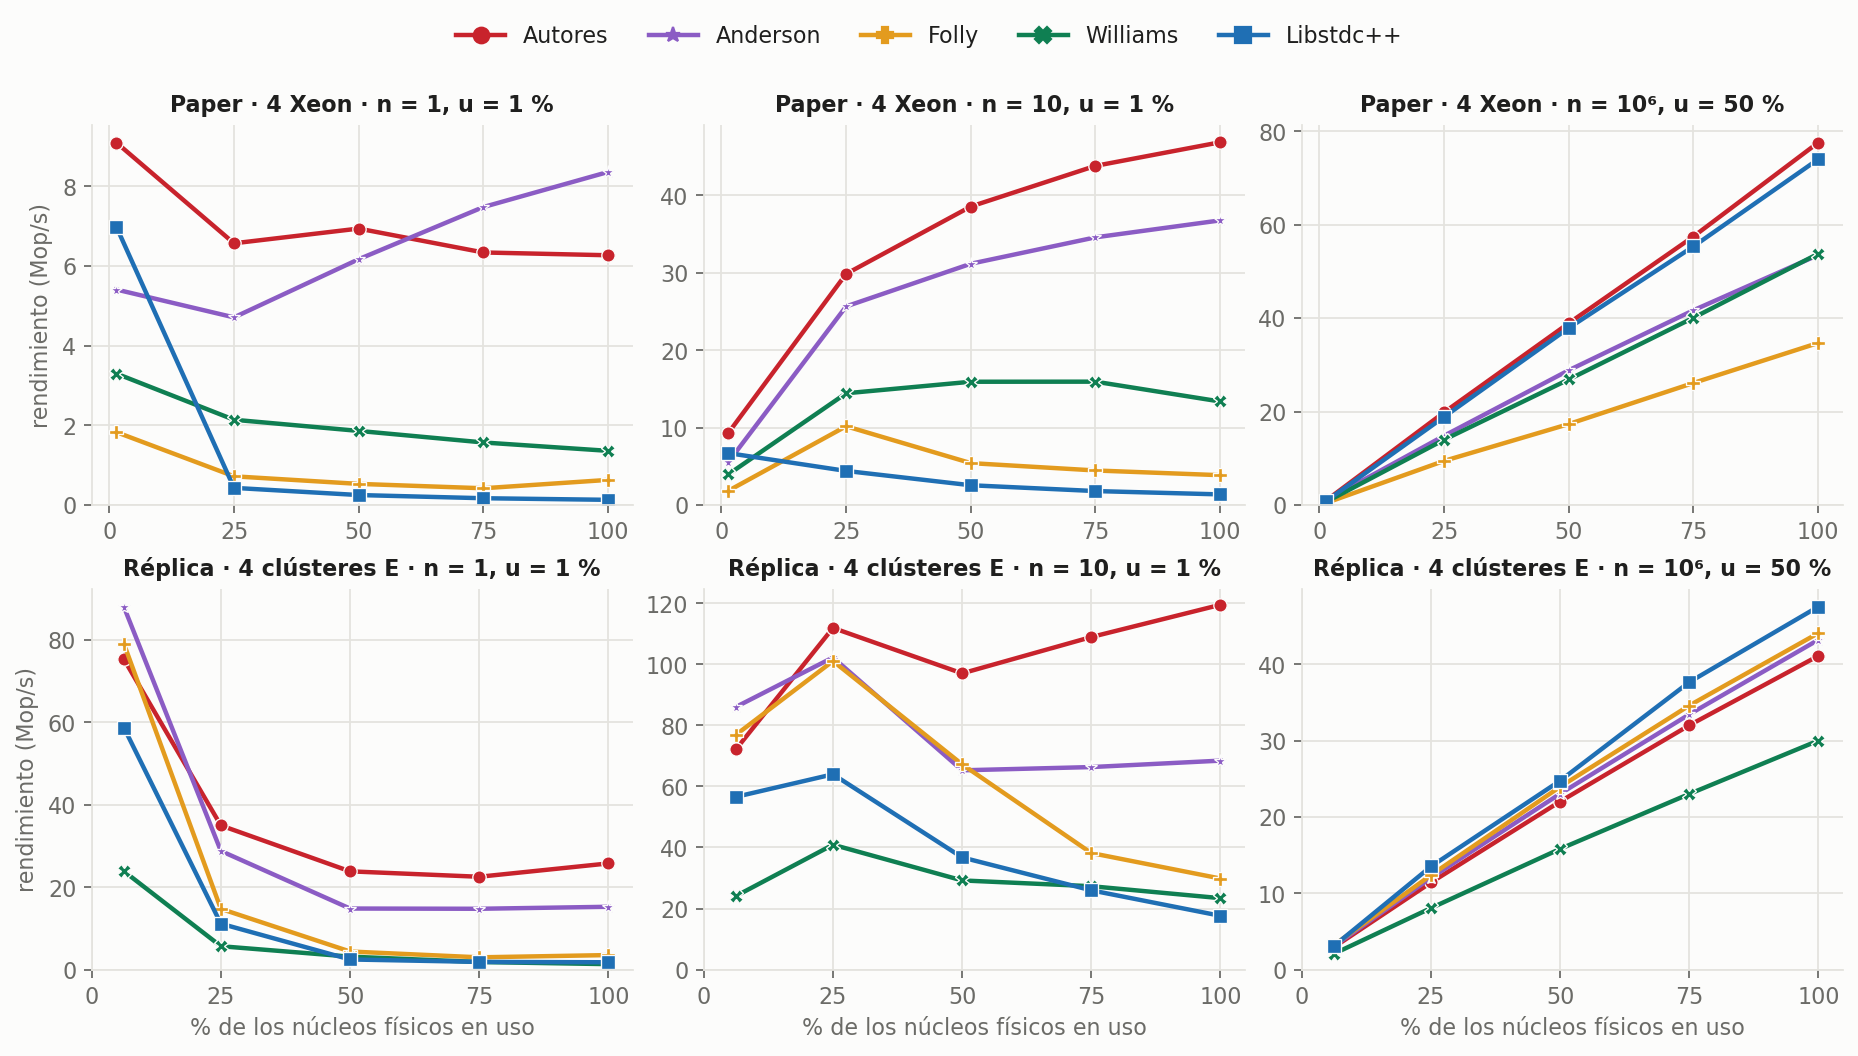
\includegraphics[width=\linewidth]{figuras/miniatura_frente_a_paper}
    \column{0.34\textwidth}
    \begin{itemize}\footnotesize\setlength{\itemsep}{3pt}
      \item $n = 10$, $u = 1$\,\%: \textcolor{verde}{\textbf{se parece}}. Autores encabeza en ambos desde el 25\,\% de la máquina.
      \item $n = \pot{6}$, $u = 50$\,\%: \textcolor{ambar}{\textbf{la forma se parece}}; cambia el orden de arriba.
      \item $n = 1$, $u = 1$\,\%: \textcolor{rojo}{\textbf{no se parece}}. En el paper Anderson sube y adelanta; aquí se queda plano.
    \end{itemize}
    \medskip
    \caja{¿Se simularon los 4 Xeon? \textbf{Solo en parte.} La física es real, pero el castigo es 1,35\por{} frente a unas 3\por, no hay NUMA y son 16 núcleos E, no 72.}
  \end{columns}
  \nota{p9_miniatura}
\end{frame}
